\section{Process' Perspective}
This perspective should clarify how code or other artifacts come from idea into the running system and everything that happens on the way.

In particular, the following descriptions should be included:

A complete description of stages and tools included in the CI/CD chains, including deployment and release of your systems.
How do you monitor your systems and what precisely do you monitor?
What do you log in your systems and how do you aggregate logs?
Brief results of the security assessment and brief description of how did you harden the security of your system based on the analysis
Applied strategy for scaling and upgrades
In case you have used AI-assistants during your project briefly explain which system(s) you used during the project and reflect how it supported/hindered your process.

%for this section see images/commit_checks,logging,monitor_bad,monitor_good
%https://codeclimate.com/github/TheisHS/test1-itu-minitwit -- link to codeclimate, everyone can see this
\subsection{CI/CD Pipeline}
\subsubsection*{Stages of the Pipeline}
\subsubsection*{Tools and Technologies}
\subsubsection*{Deployment and Release Processes}
Docker, feb 29
\subsection{System Monitoring and Logging}
\subsubsection*{Monitoring Strategies and Tools}
%march 8,12,13 (check lecture notes for reactive vs proactive monitoring and what we have done)
In managing our system's health, we rely on two key tools: Prometheus and Grafana. Prometheus is a push/pull-hybrid whitebox monitoring system from which our instrumented application pushes our defined metrics, which are then pulled/scraped by the Prometheus central system... (ik færdig/skriv om/tilføj flere ligegyldige termer fra monitoring forelæsningen)\\

Grafana is an open-source platform used for visualising and analysing time-series data. In our setup, we use Grafana as a dashboarding tool that uses our Prometheus server as the primary data source for monitoring. This allows us to create dashboards that provide real-time insights of our measures.\\
%Reactive Monitoring: In reactive monitoring, the focus is on responding to issues after they occur.
%Proactive Monitoring: Proactive monitoring involves anticipating and preventing issues before they impact the system.

As from the Monitoring Maturity Model by James Turnbull\cite{MonitoringMaturityModel}, our monitoring strategy combines proactive elements, such as monitoring uptime and tracking error rates metrics to anticipate and prevent issues, with reactive elements, such as tracking specific error codes and status of specific user requests to respond promptly to any issues that arise.

\subsubsection*{Key Metrics Monitored}
We have defined monitoring metrics for both the API and the web client. However, given the API's consistent workload from the simulation, this has been our primary focus. We have defined a total of 14 metrics for the API:
\begin{multicols}{2}
\begin{itemize}
    \item \textbf{http\_requests\_total}
    \item \textbf{database\_accesses\_total}
    \item \textbf{errors\_total}
    \item \textbf{get\_user\_id\_requests}
    \item \textbf{get\_user\_id\_requests\_failed}
    \item \textbf{follow\_requests}
    \item \textbf{follow\_requests\_failed}
    \item \textbf{unfollow\_requests}
    \item \textbf{unfollow\_requests\_failed}
    \item \textbf{post\_message\_requests}
    \item \textbf{post\_message\_requests\_failed}
    \item \textbf{not\_found}
    \item \textbf{bad\_request}
    \item \textbf{internal\_server\_error}
\end{itemize}
\end{multicols}

These monitoring metrics are visualised in a Grafana dashboard named \texttt{Minitwit\_Dashboard} as shown in Figure \ref{fig:monitor_good}. 

\begin{figure}[H]
    \centering
    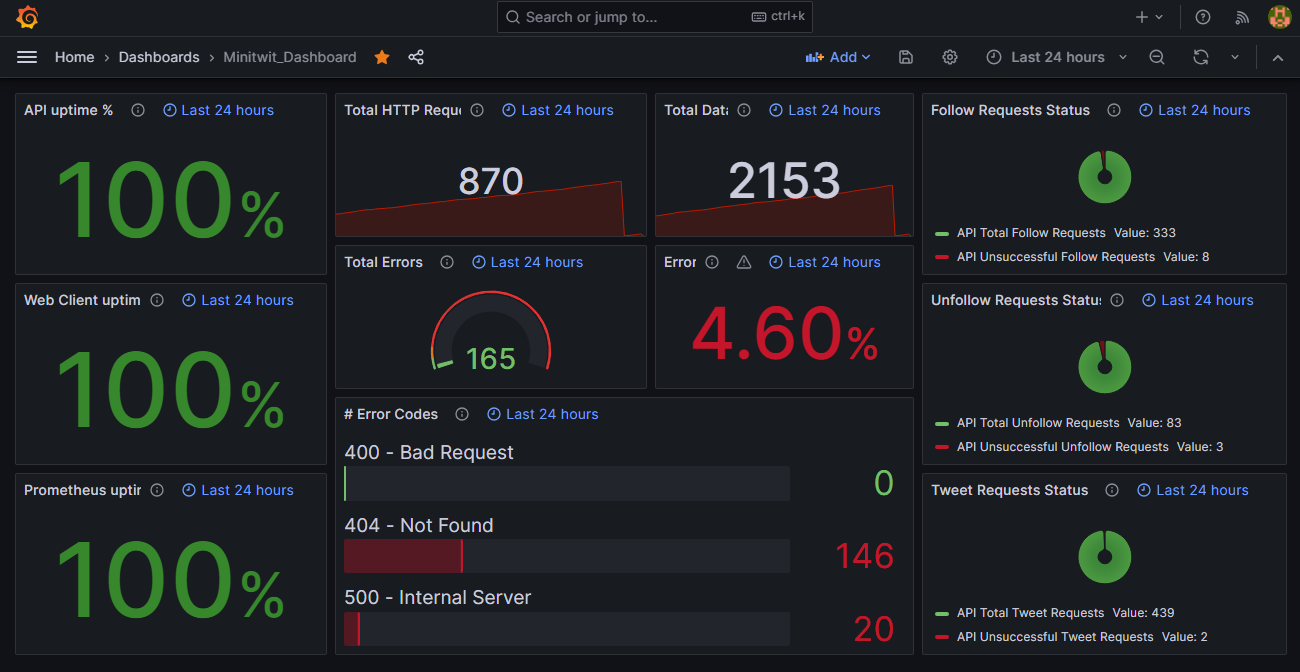
\includegraphics[width=0.8\textwidth]{images/monitor_good.png}
    \caption{Minitwit\_Dashboard - API Monitoring}
    \label{fig:monitor_good}
\end{figure}
The key metrics are categorised and displayed as follows:

\textbf{Total HTTP requests and Database accesses}, \textbf{Total Errors and Error Ratio}, \textbf{Error code distribution} of the total errors, and \textbf{Specific user request success/failure} (follow, unfollow, tweet). 

Additionally, the visualisation shows the uptime percentage of the API, Web Client, and Prometheus, which is derived from predefined Prometheus metrics.

\subsubsection*{Log Aggregation Techniques}
april 1, mention log rotation, possibly mention that we also tried setting up ELK at first
\subsection{Security Assessment}
\subsubsection*{Assessment Results}
\subsubsection*{Security Hardening Approaches}
\subsection{Scaling and Upgrade Strategy}
april 23
%\subsection{AI Tools Utilized}